\documentclass[conference]{IEEEtran}
\IEEEoverridecommandlockouts
% The preceding line is only needed to identify funding in the first footnote. If that is unneeded, please comment it out.
\usepackage{cite}
\usepackage{amsmath,amssymb,amsfonts}
\usepackage{algorithmic}
\usepackage{graphicx}
\usepackage{textcomp}
\usepackage{xcolor}
\def\BibTeX{{\rm B\kern-.05em{\sc i\kern-.025em b}\kern-.08em
    T\kern-.1667em\lower.7ex\hbox{E}\kern-.125emX}}


\usepackage{tikz}
\usetikzlibrary{calc}
\usetikzlibrary{arrows.meta}

\begin{document}

\title{Adaptive Multi-Agent Programming with Programs and Promises
(Doctoral Symposium)}

\author{\IEEEauthorblockN{Oleks Shturmov}
\IEEEauthorblockA{\textit{Department of Informatics} \\
\textit{University of Oslo}\\
Norway \\
\texttt{oleks@oleks.info}}
% \and
% \IEEEauthorblockN{2\textsuperscript{nd} Given Name Surname}
% \IEEEauthorblockA{\textit{dept. name of organization (of Aff.)} \\
% \textit{name of organization (of Aff.)}\\
% City, Country \\
% email address or ORCID}
% \and
% \IEEEauthorblockN{3\textsuperscript{rd} Given Name Surname}
% \IEEEauthorblockA{\textit{dept. name of organization (of Aff.)} \\
% \textit{name of organization (of Aff.)}\\
% City, Country \\
% email address or ORCID}
% \and
% \IEEEauthorblockN{4\textsuperscript{th} Given Name Surname}
% \IEEEauthorblockA{\textit{dept. name of organization (of Aff.)} \\
% \textit{name of organization (of Aff.)}\\
% City, Country \\
% email address or ORCID}
% \and
% \IEEEauthorblockN{5\textsuperscript{th} Given Name Surname}
% \IEEEauthorblockA{\textit{dept. name of organization (of Aff.)} \\
% \textit{name of organization (of Aff.)}\\
% City, Country \\
% email address or ORCID}
% \and
% \IEEEauthorblockN{6\textsuperscript{th} Given Name Surname}
% \IEEEauthorblockA{\textit{dept. name of organization (of Aff.)} \\
% \textit{name of organization (of Aff.)}\\
% City, Country \\
% email address or ORCID}
}

\maketitle

\begin{abstract}

% Programming adaptive systems, composed of physically distributed
% agents, entails programming the adaptation logic of the individual
% agents.

Agents that adapt their behavior in response to communicative events
by other agents, can be viewed as machines that can be programmed by
those other agents. At the time same time, such agents can be viewed
as machines that each deliver a promise to behave a certain way, until
given conditions change. This work explores the potential benefits for
the programmer in taking this perspective, when programming multiple,
adaptive, physically distributed agents, engaged in a common
objective.

\end{abstract}

\begin{IEEEkeywords}
adaptive, multi-agent, distributed, programming
\end{IEEEkeywords}

\section{Motivation and Challenges}

\emph{TASK: explain why this research is important, and identify the
key research question(s) and challenges that have yet to be addressed
by the community - including limitations of current approaches.}

Contemporary distributed systems communication primitives tend to deal
in short-term planning horizons. For instance, while an inquiry about
the state of an agent may resolve to a particular response, its state
may be subject to fast-paced change, when compared with the time it
takes to communicate across the network. This renders the response
relevant only for a short period of time, if at all, when delivered.
Follow-up requests will be relevant for an even shorter period of
time.

Uncontested this leads to either high failure rates of follow-up
requests, or highly congested networks. In particular, the state of a
remote agent may be ill-predictable, while short-sighted status
messages have little positive impact on the expected success rate of
follow-up messages. Hence, we may choose to flood the network in
attempt to keep track of the fast-paced changes, while still gaining
little confidence that we can act on those changes in due time.

% At the same time, agents in highly dynamic systems often cannot freeze
% in anticipation of follow-up requests.

As a particular example, consider the following multi-agent problem: 3
robots roam a fixed-size room, looking for tasks to do. A task can be
solved by 2 robots getting within radius $\omega$ of the task. Tasks
appear at random, in random positions, and neither move, nor disappear
until solved. Agents have an omnidirectional field of sight with
radius $\omega$, and can communicate by broadcasting messages within
radius $\beta$, where $\beta>\omega$. The robots roam around, calling
out for help from other agents whenever they see a task.

\begin{figure}
\centering
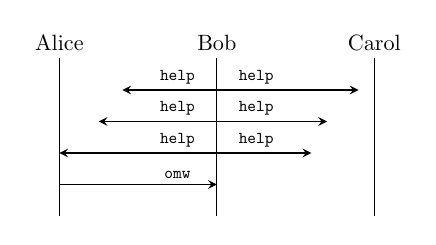
\begin{tikzpicture}
  \coordinate (a) at (0,0);
  \coordinate (b) at (0,2);
  \coordinate (c) at (2,0);
  \coordinate (d) at (2,2);
  \coordinate (e) at (4,0);
  \coordinate (f) at (4,2);
  \draw %
    (a) -- (b)node[pos=1.1,scale=0.8]{Alice}%
    (c) -- (d)node[pos=1.1,scale=0.8]{Bob}%
    (e) -- (f)node[pos=1.1,scale=0.8]{Carol};
  \draw[stealth-,shorten <=8mm] %
    ($(a)!0.8!(b)$) -- node[above,near end,scale=0.6]{\texttt{help}}($(c)!0.8!(d)$);
  \draw[stealth-,shorten <=5mm] %
    ($(a)!0.6!(b)$) -- node[above,near end,scale=0.6]{\texttt{help}}($(c)!0.6!(d)$);
  \draw[stealth-] %
    ($(a)!0.4!(b)$) -- node[above,near end,scale=0.6]{\texttt{help}}($(c)!0.4!(d)$);

  \draw[-stealth] %
    ($(a)!0.2!(b)$) -- node[above,near end,scale=0.6]{\texttt{omw}}($(c)!0.2!(d)$);

  \draw[stealth-,shorten <=2mm] %
    ($(e)!0.8!(f)$) -- node[above,near end,scale=0.6]{\texttt{help}}($(c)!0.8!(d)$);
  \draw[stealth-,shorten <=6mm] %
    ($(e)!0.6!(f)$) -- node[above,near end,scale=0.6]{\texttt{help}}($(c)!0.6!(d)$);
  \draw[stealth-,shorten <=8mm] %
    ($(e)!0.4!(f)$) -- node[above,near end,scale=0.6]{\texttt{help}}($(c)!0.4!(d)$);

\end{tikzpicture}
\caption{Sequence diagram illustrating Bob's calls out for
\texttt{help}, as Alice moves closer to Bob, while Carol moves away.}
\label{fig1}
\end{figure}

Figure \ref{fig1} showcases 3 robots, Alice, Bob, and Carol, where Bob
has found a task and calls out to Alice and Carol for help. As Alice
and Carol also roam about the room, they may be out of reach for Bob's
broadcasting signal.

\section{Contribution and Objectives}

\emph{TASK: present the main contribution of the research in a way
that a non-expert could clearly understand, then present the detailed
objectives of your research, highlighting why your work is novel in
comparison to existing research.}

To expand the relevance horizon of our messages, consider: (1)
constructing responses such that they give an indication of not just
the current state of an agent, but also its possible future states,
and/or (2) composing follow-up requests such that they can be serviced
successfully, despite possible meanwhile state changes at the remote
agent.

To this end, both requests and responses may employ sentences in a
linear temporal logic, a logic that deals with truth of propositions
over time\cite{2022-Live-Synthesis}.


% 2
% vacuuming and 1 polishing robot roam a fixed-size room looking for
% tasks to do---spots to vacuum and polish. A task spawns at a random
% point in time, at a random position, and neither moves, nor disappears
% until a vacuuming and polishing robot get within radius $\omega$ of
% the task and solve it.

% It seems safe to conjecture that an approach to communication that
% seeks to increase the expected success rate of follow-up requests
% would lead to less congested network traffic.

\section{Methodology and Preliminary Results}

\emph{TASK: present the methodology of your approach, discussing why
it is suitable to your contribution, and also present any preliminary
results if you have them, including a statement about the current
status of your work.}

\section{Future and Research Plan}

\emph{TASK: summarise your intended future work and provide a schedule
of milestones with a discussion of their feasibility.}

\bibliographystyle{IEEEtran}
\bibliography{references}

\end{document}
